\documentclass[twoside]{book}

% Packages required by doxygen
\usepackage{calc}
\usepackage{doxygen}
\usepackage{graphicx}
\usepackage[utf8]{inputenc}
\usepackage{makeidx}
\usepackage{multicol}
\usepackage{multirow}
\usepackage{textcomp}
\usepackage[table]{xcolor}

% Font selection
\usepackage[T1]{fontenc}
\usepackage{mathptmx}
\usepackage[scaled=.90]{helvet}
\usepackage{courier}
\usepackage{amssymb}
\usepackage{sectsty}
\renewcommand{\familydefault}{\sfdefault}
\allsectionsfont{%
  \fontseries{bc}\selectfont%
  \color{darkgray}%
}
\renewcommand{\DoxyLabelFont}{%
  \fontseries{bc}\selectfont%
  \color{darkgray}%
}

% Page & text layout
\usepackage{geometry}
\geometry{%
  a4paper,%
  top=2.5cm,%
  bottom=2.5cm,%
  left=2.5cm,%
  right=2.5cm%
}
\tolerance=750
\hfuzz=15pt
\hbadness=750
\setlength{\emergencystretch}{15pt}
\setlength{\parindent}{0cm}
\setlength{\parskip}{0.2cm}
\makeatletter
\renewcommand{\paragraph}{%
  \@startsection{paragraph}{4}{0ex}{-1.0ex}{1.0ex}{%
    \normalfont\normalsize\bfseries\SS@parafont%
  }%
}
\renewcommand{\subparagraph}{%
  \@startsection{subparagraph}{5}{0ex}{-1.0ex}{1.0ex}{%
    \normalfont\normalsize\bfseries\SS@subparafont%
  }%
}
\makeatother

% Headers & footers
\usepackage{fancyhdr}
\pagestyle{fancyplain}
\fancyhead[LE]{\fancyplain{}{\bfseries\thepage}}
\fancyhead[CE]{\fancyplain{}{}}
\fancyhead[RE]{\fancyplain{}{\bfseries\leftmark}}
\fancyhead[LO]{\fancyplain{}{\bfseries\rightmark}}
\fancyhead[CO]{\fancyplain{}{}}
\fancyhead[RO]{\fancyplain{}{\bfseries\thepage}}
\fancyfoot[LE]{\fancyplain{}{}}
\fancyfoot[CE]{\fancyplain{}{}}
\fancyfoot[RE]{\fancyplain{}{\bfseries\scriptsize 2016年01月22日(金) 22時20分26秒作成 -\/ E\-V3\-Control\-Server / 構成\-:  Doxygen }}
\fancyfoot[LO]{\fancyplain{}{\bfseries\scriptsize 2016年01月22日(金) 22時20分26秒作成 -\/ E\-V3\-Control\-Server / 構成\-:  Doxygen }}
\fancyfoot[CO]{\fancyplain{}{}}
\fancyfoot[RO]{\fancyplain{}{}}
\renewcommand{\footrulewidth}{0.4pt}
\renewcommand{\chaptermark}[1]{%
  \markboth{#1}{}%
}
\renewcommand{\sectionmark}[1]{%
  \markright{\thesection\ #1}%
}

% Indices & bibliography
\usepackage{natbib}
\usepackage[titles]{tocloft}
\setcounter{tocdepth}{3}
\setcounter{secnumdepth}{5}
\makeindex

% Custom commands
\newcommand{\clearemptydoublepage}{%
  \newpage{\pagestyle{empty}\cleardoublepage}%
}


%===== C O N T E N T S =====

\begin{document}

% Titlepage & ToC
\pagenumbering{roman}
\begin{titlepage}
\vspace*{7cm}
\begin{center}%
{\Large E\-V3\-Control\-Server }\\
\vspace*{1cm}
{\large 構築\-: Doxygen 1.8.6}\\
\vspace*{0.5cm}
{\small 2016年01月22日(金) 22時20分26秒}\\
\end{center}
\end{titlepage}
\clearemptydoublepage
\tableofcontents
\clearemptydoublepage
\pagenumbering{arabic}

%--- Begin generated contents ---
\chapter{階層索引}
\section{クラス階層}
クラス階層一覧です。大雑把に文字符号順で並べられています。\begin{DoxyCompactList}
\item \contentsline{section}{E\-V3\-Control\-Server}{\pageref{class_e_v3_control_server}}{}
\item \contentsline{section}{Read\-File}{\pageref{class_read_file}}{}
\item \contentsline{section}{Socket\-Server}{\pageref{class_socket_server}}{}
\item Timer\-Task\begin{DoxyCompactList}
\item \contentsline{section}{Run\-Server}{\pageref{class_run_server}}{}
\end{DoxyCompactList}
\end{DoxyCompactList}

\chapter{クラス索引}
\section{クラス一覧}
クラス・構造体・共用体・インターフェースの一覧です。\begin{DoxyCompactList}
\item\contentsline{section}{{\bf E\-V3\-Control\-Server} \\*サーバー側のメインの処理クラス }{\pageref{class_e_v3_control_server}}{}
\item\contentsline{section}{{\bf Read\-File} \\*ファイルを読み込むクラス }{\pageref{class_read_file}}{}
\item\contentsline{section}{{\bf Run\-Server} \\*サーバー側で連続で行う処理を記述したクラス }{\pageref{class_run_server}}{}
\item\contentsline{section}{{\bf Socket\-Server} \\*ソケット通信のサーバー側クラス }{\pageref{class_socket_server}}{}
\end{DoxyCompactList}

\chapter{ファイル索引}
\section{ファイル一覧}
ファイル一覧です。\begin{DoxyCompactList}
\item\contentsline{section}{{\bf E\-V3\-Control\-Server.\-java} \\*E\-V3を制御するクライアント(\-P\-C)側のメインクラス. }{\pageref{_e_v3_control_server_8java}}{}
\item\contentsline{section}{{\bf Read\-File.\-java} \\*ファイル読み込みクラス.\-Kinectが生成したファイルを読み込む }{\pageref{_read_file_8java}}{}
\item\contentsline{section}{{\bf Run\-Server.\-java} \\*サーバー(\-P\-C)側の時間をスケジューリングするクラス. }{\pageref{_run_server_8java}}{}
\item\contentsline{section}{{\bf Socket\-Server.\-java} \\*サーバークラス.\-E\-V3からの通信を\-P\-C側で受け取る }{\pageref{_socket_server_8java}}{}
\end{DoxyCompactList}

\chapter{クラス詳解}
\section{E\-V3\-Control\-Server クラス}
\label{class_e_v3_control_server}\index{E\-V3\-Control\-Server@{E\-V3\-Control\-Server}}


サーバー側のメインの処理クラス  


\subsection*{静的公開メンバ関数}
\begin{DoxyCompactItemize}
\item 
static void {\bf main} (String[$\,$] args)
\begin{DoxyCompactList}\small\item\em メインメソッド \end{DoxyCompactList}\end{DoxyCompactItemize}


\subsection{詳解}
サーバー側のメインの処理クラス 

 E\-V3\-Control\-Server.\-java の 15 行目に定義があります。



\subsection{メソッド詳解}
\index{E\-V3\-Control\-Server@{E\-V3\-Control\-Server}!main@{main}}
\index{main@{main}!EV3ControlServer@{E\-V3\-Control\-Server}}
\subsubsection[{main}]{\setlength{\rightskip}{0pt plus 5cm}static void E\-V3\-Control\-Server.\-main (
\begin{DoxyParamCaption}
\item[{String[$\,$]}]{args}
\end{DoxyParamCaption}
)\hspace{0.3cm}{\ttfamily [static]}}\label{class_e_v3_control_server_abf47157f3238d6573639e578d7d77492}


メインメソッド 



 E\-V3\-Control\-Server.\-java の 19 行目に定義があります。



このクラス詳解は次のファイルから抽出されました\-:\begin{DoxyCompactItemize}
\item 
{\bf E\-V3\-Control\-Server.\-java}\end{DoxyCompactItemize}

\section{Read\-File クラス}
\label{class_read_file}\index{Read\-File@{Read\-File}}


ファイルを読み込むクラス  


\subsection*{公開メンバ関数}
\begin{DoxyCompactItemize}
\item 
void {\bf Read\-Velocity\-Yaw\-File} (String args[$\,$])
\begin{DoxyCompactList}\small\item\em ファイルを読み込むメソッド \end{DoxyCompactList}\end{DoxyCompactItemize}
\subsection*{公開変数類}
\begin{DoxyCompactItemize}
\item 
double {\bf velocity}
\begin{DoxyCompactList}\small\item\em 速度 \end{DoxyCompactList}\item 
double {\bf yaw}
\begin{DoxyCompactList}\small\item\em ヨー角 \end{DoxyCompactList}\end{DoxyCompactItemize}


\subsection{詳解}
ファイルを読み込むクラス 

 Read\-File.\-java の 14 行目に定義があります。



\subsection{メソッド詳解}
\index{Read\-File@{Read\-File}!Read\-Velocity\-Yaw\-File@{Read\-Velocity\-Yaw\-File}}
\index{Read\-Velocity\-Yaw\-File@{Read\-Velocity\-Yaw\-File}!ReadFile@{Read\-File}}
\subsubsection[{Read\-Velocity\-Yaw\-File}]{\setlength{\rightskip}{0pt plus 5cm}void Read\-File.\-Read\-Velocity\-Yaw\-File (
\begin{DoxyParamCaption}
\item[{String}]{args[$\,$]}
\end{DoxyParamCaption}
)}\label{class_read_file_ac947af61d03b31192680172cf742bad8}


ファイルを読み込むメソッド 


\begin{DoxyParams}{引数}
{\em args\mbox{[}$\,$\mbox{]}} & String型 \\
\hline
\end{DoxyParams}


 Read\-File.\-java の 24 行目に定義があります。



参照先 velocity, yaw.



\subsection{メンバ詳解}
\index{Read\-File@{Read\-File}!velocity@{velocity}}
\index{velocity@{velocity}!ReadFile@{Read\-File}}
\subsubsection[{velocity}]{\setlength{\rightskip}{0pt plus 5cm}double Read\-File.\-velocity}\label{class_read_file_a9389e007e9ee86d18f29e5117f5d5d63}


速度 



 Read\-File.\-java の 16 行目に定義があります。



参照元 Read\-Velocity\-Yaw\-File().

\index{Read\-File@{Read\-File}!yaw@{yaw}}
\index{yaw@{yaw}!ReadFile@{Read\-File}}
\subsubsection[{yaw}]{\setlength{\rightskip}{0pt plus 5cm}double Read\-File.\-yaw}\label{class_read_file_afb5e582fdf100eba04ef789b0803dcb7}


ヨー角 



 Read\-File.\-java の 17 行目に定義があります。



参照元 Read\-Velocity\-Yaw\-File().



このクラス詳解は次のファイルから抽出されました\-:\begin{DoxyCompactItemize}
\item 
{\bf Read\-File.\-java}\end{DoxyCompactItemize}

\section{Run\-Server クラス}
\label{class_run_server}\index{Run\-Server@{Run\-Server}}


サーバー側で連続で行う処理を記述したクラス  




Run\-Server の継承関係図\nopagebreak
\begin{figure}[H]
\begin{center}
\leavevmode
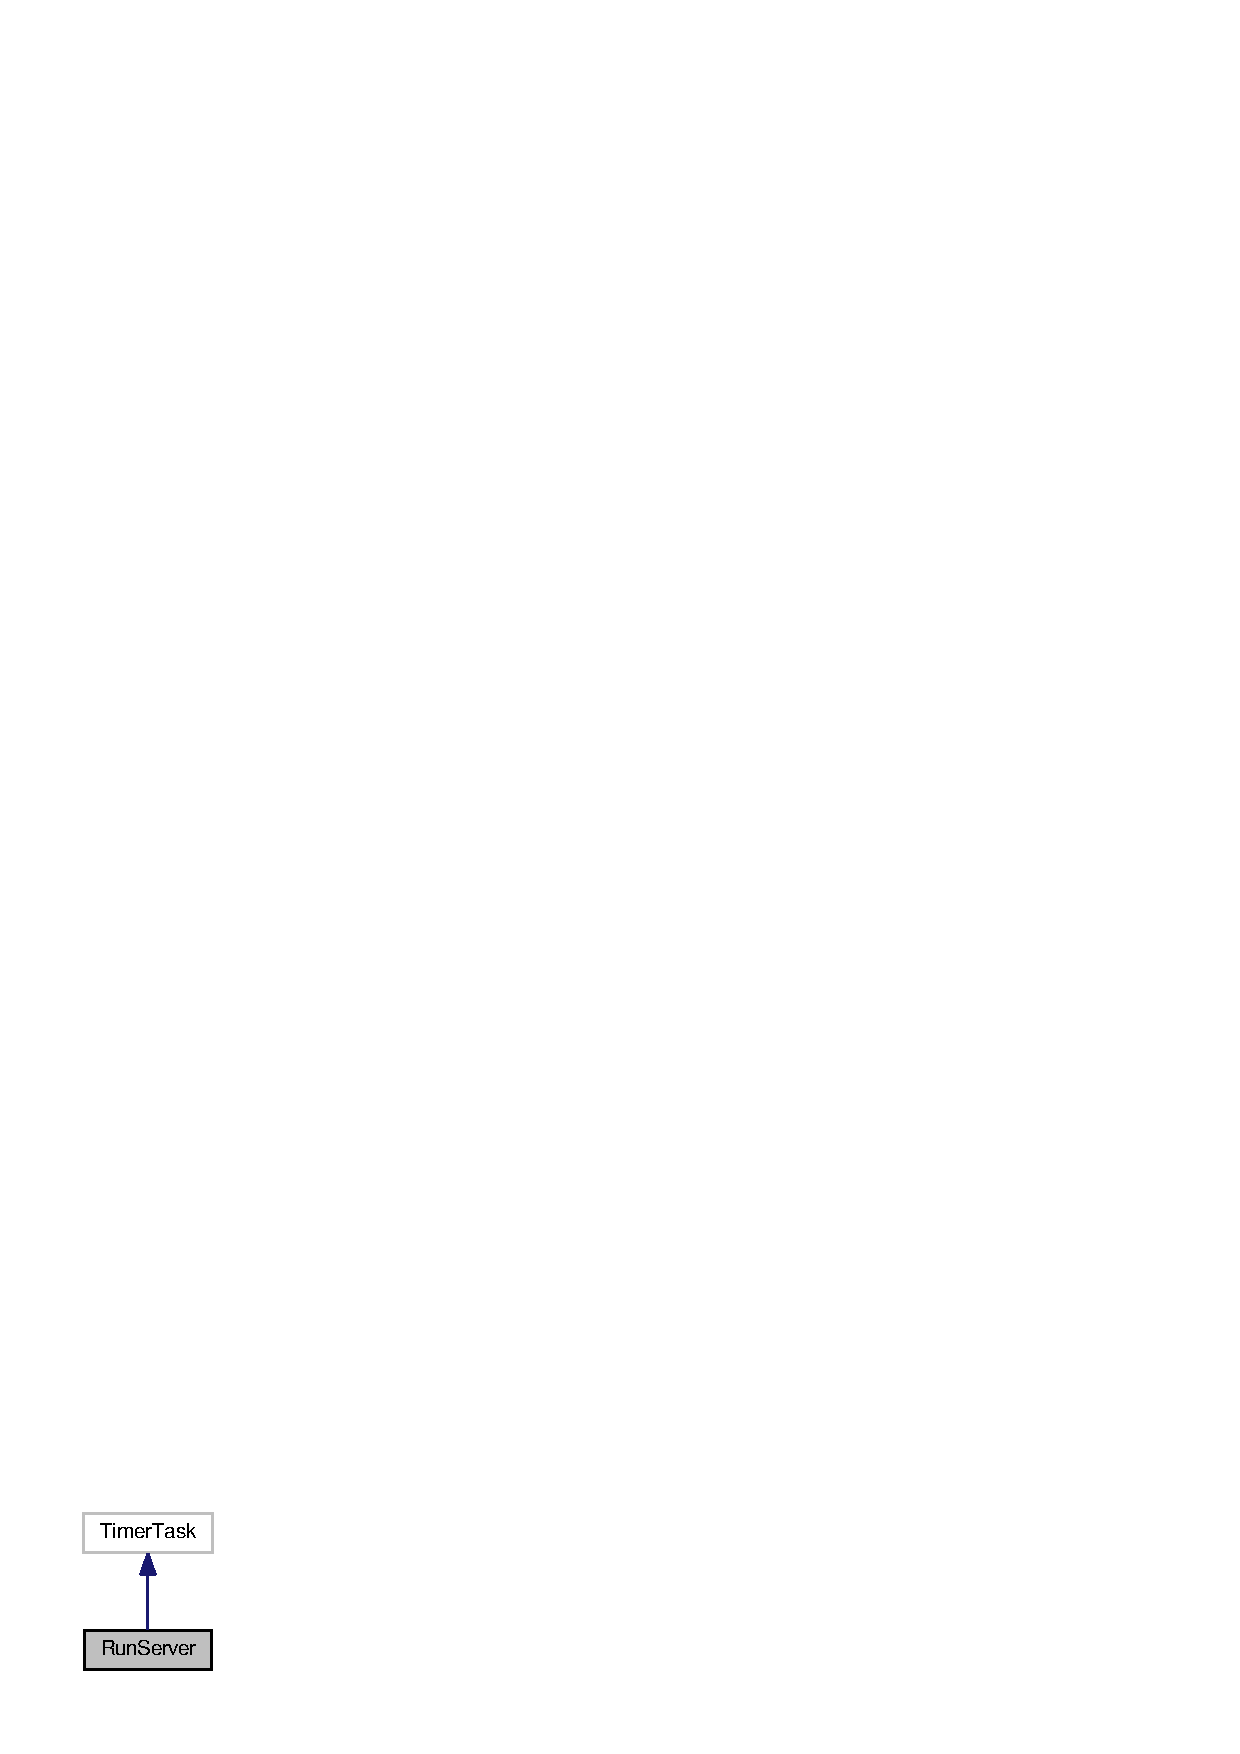
\includegraphics[width=106pt]{class_run_server__inherit__graph}
\end{center}
\end{figure}


Run\-Server 連携図
\nopagebreak
\begin{figure}[H]
\begin{center}
\leavevmode
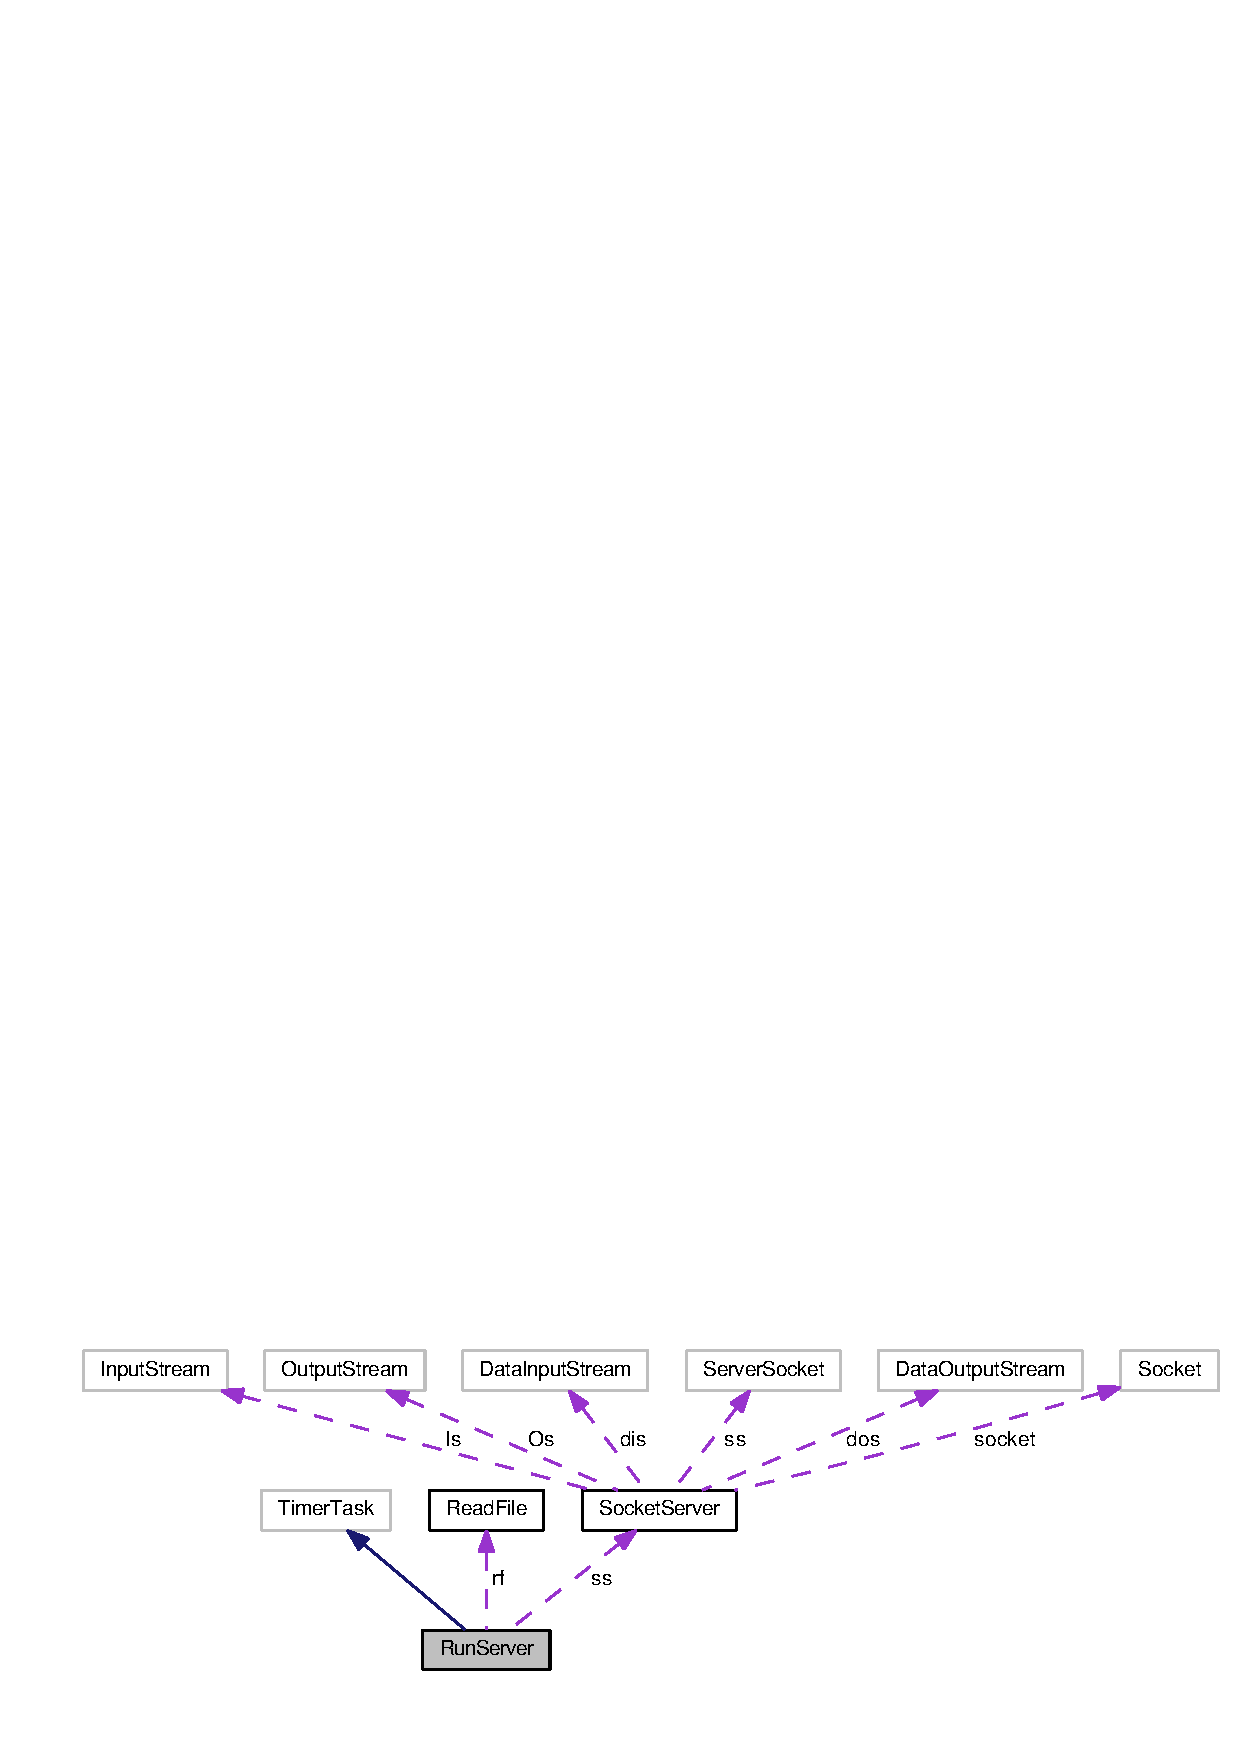
\includegraphics[width=350pt]{class_run_server__coll__graph}
\end{center}
\end{figure}
\subsection*{公開メンバ関数}
\begin{DoxyCompactItemize}
\item 
void {\bf run} ()
\begin{DoxyCompactList}\small\item\em \doxyref{run()}{p.}{class_run_server_aad333a6b0041adaf2ca0de7abb739819}.処理の流れをここに書く \end{DoxyCompactList}\end{DoxyCompactItemize}


\subsection{詳解}
サーバー側で連続で行う処理を記述したクラス 

 Run\-Server.\-java の 16 行目に定義があります。



\subsection{メソッド詳解}
\index{Run\-Server@{Run\-Server}!run@{run}}
\index{run@{run}!RunServer@{Run\-Server}}
\subsubsection[{run}]{\setlength{\rightskip}{0pt plus 5cm}void Run\-Server.\-run (
\begin{DoxyParamCaption}
{}
\end{DoxyParamCaption}
)}\label{class_run_server_aad333a6b0041adaf2ca0de7abb739819}


\doxyref{run()}{p.}{class_run_server_aad333a6b0041adaf2ca0de7abb739819}.処理の流れをここに書く 



 Run\-Server.\-java の 35 行目に定義があります。



このクラス詳解は次のファイルから抽出されました\-:\begin{DoxyCompactItemize}
\item 
{\bf Run\-Server.\-java}\end{DoxyCompactItemize}

\section{Socket\-Server クラス}
\label{class_socket_server}\index{Socket\-Server@{Socket\-Server}}


ソケット通信のサーバー側クラス  




Socket\-Server 連携図\nopagebreak
\begin{figure}[H]
\begin{center}
\leavevmode
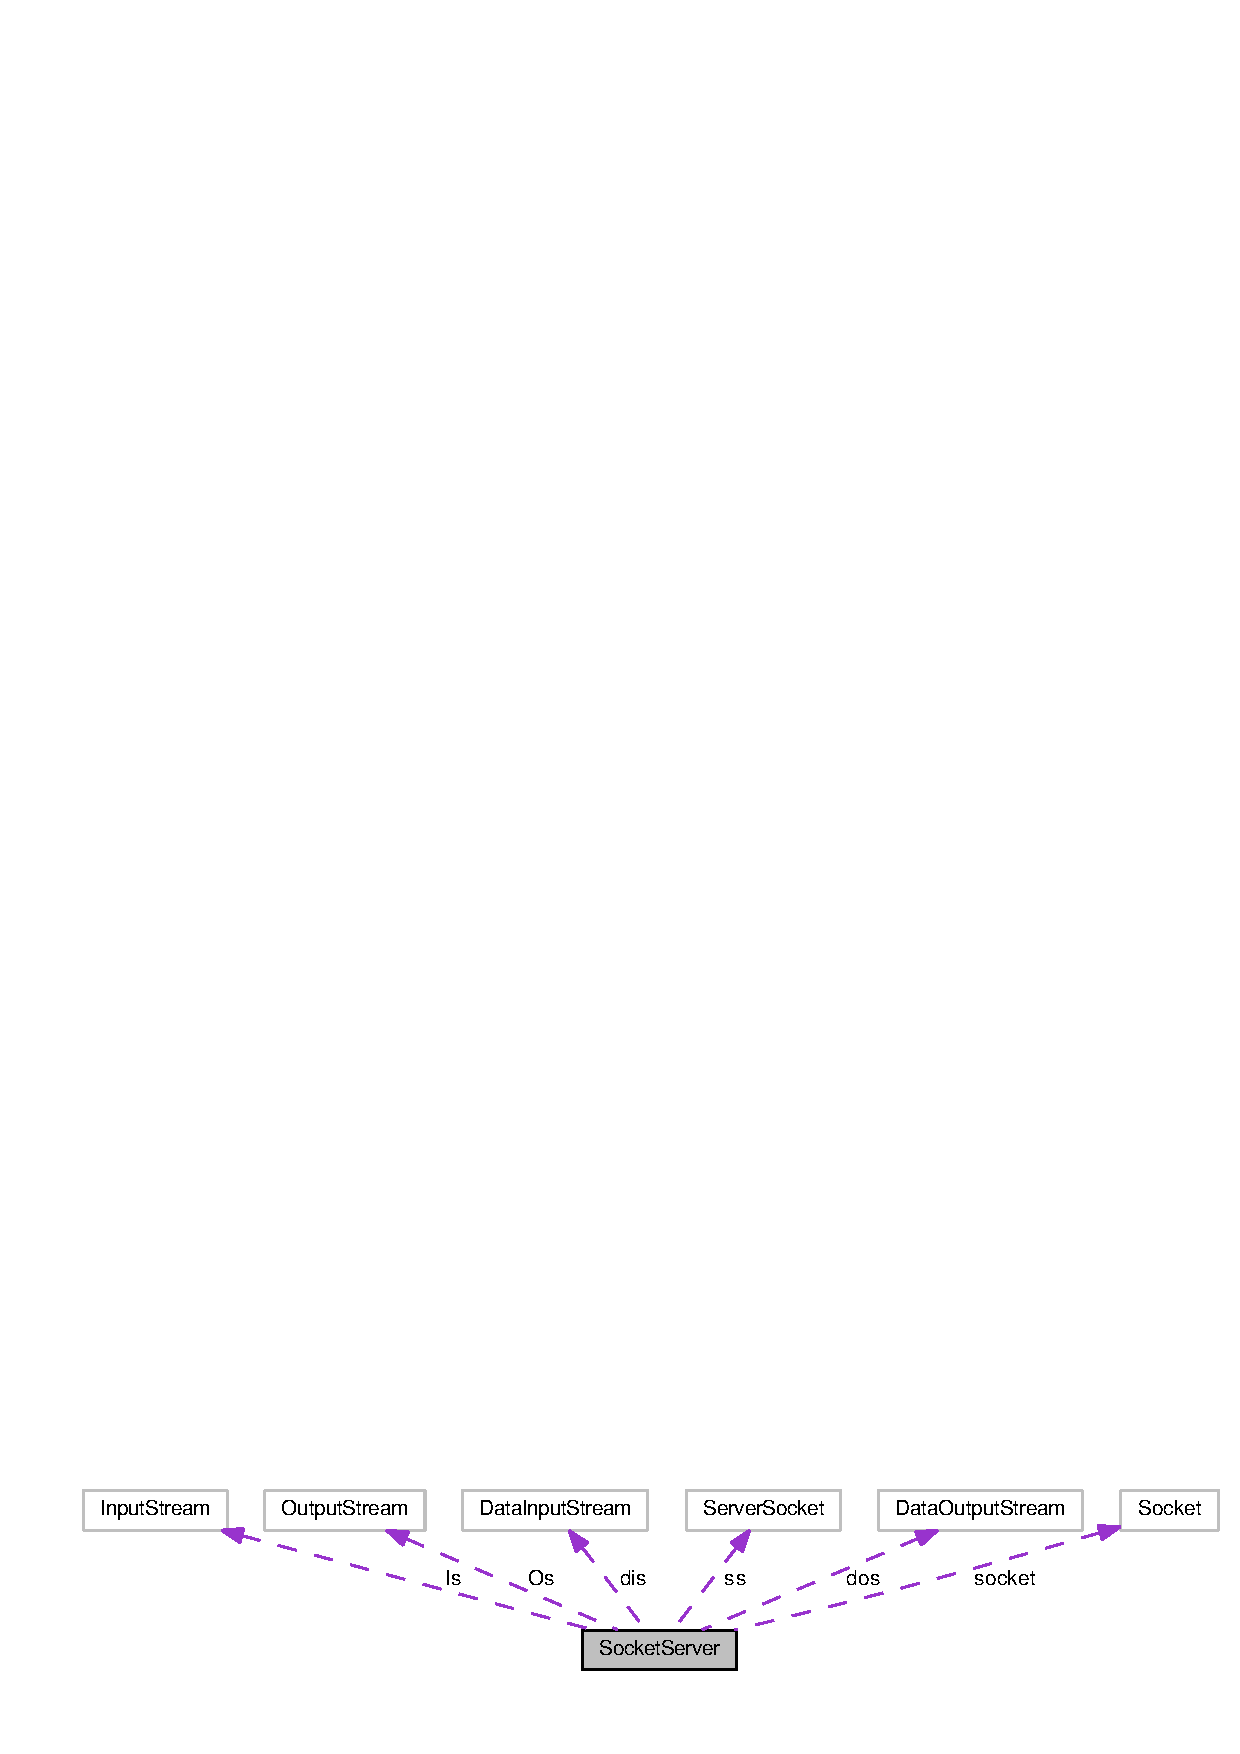
\includegraphics[width=350pt]{class_socket_server__coll__graph}
\end{center}
\end{figure}
\subsection*{公開メンバ関数}
\begin{DoxyCompactItemize}
\item 
void {\bf Make\-Connection} (String args[$\,$])
\begin{DoxyCompactList}\small\item\em コネクションをはるメソッド \end{DoxyCompactList}\item 
void {\bf Send\-Data} (double velocity, double yaw)
\begin{DoxyCompactList}\small\item\em データを送信するメソッド \end{DoxyCompactList}\end{DoxyCompactItemize}


\subsection{詳解}
ソケット通信のサーバー側クラス 

 Socket\-Server.\-java の 20 行目に定義があります。



\subsection{メソッド詳解}
\index{Socket\-Server@{Socket\-Server}!Make\-Connection@{Make\-Connection}}
\index{Make\-Connection@{Make\-Connection}!SocketServer@{Socket\-Server}}
\subsubsection[{Make\-Connection}]{\setlength{\rightskip}{0pt plus 5cm}void Socket\-Server.\-Make\-Connection (
\begin{DoxyParamCaption}
\item[{String}]{args[$\,$]}
\end{DoxyParamCaption}
)}\label{class_socket_server_a667dedaab35c1f72f21b062c22e70c94}


コネクションをはるメソッド 

  

 Socket\-Server.\-java の 34 行目に定義があります。

\index{Socket\-Server@{Socket\-Server}!Send\-Data@{Send\-Data}}
\index{Send\-Data@{Send\-Data}!SocketServer@{Socket\-Server}}
\subsubsection[{Send\-Data}]{\setlength{\rightskip}{0pt plus 5cm}void Socket\-Server.\-Send\-Data (
\begin{DoxyParamCaption}
\item[{double}]{velocity, }
\item[{double}]{yaw}
\end{DoxyParamCaption}
)}\label{class_socket_server_abdfc0aed70a5e6527f72de2476ce24af}


データを送信するメソッド 



 Socket\-Server.\-java の 53 行目に定義があります。



このクラス詳解は次のファイルから抽出されました\-:\begin{DoxyCompactItemize}
\item 
{\bf Socket\-Server.\-java}\end{DoxyCompactItemize}

\chapter{ファイル詳解}
\section{E\-V3\-Control\-Server.\-java ファイル}
\label{_e_v3_control_server_8java}\index{E\-V3\-Control\-Server.\-java@{E\-V3\-Control\-Server.\-java}}


E\-V3を制御するクライアント(\-P\-C)側のメインクラス.  


\subsection*{クラス}
\begin{DoxyCompactItemize}
\item 
class {\bf E\-V3\-Control\-Server}
\begin{DoxyCompactList}\small\item\em サーバー側のメインの処理クラス \end{DoxyCompactList}\end{DoxyCompactItemize}


\subsection{詳解}
E\-V3を制御するクライアント(\-P\-C)側のメインクラス. \begin{DoxyDate}{日付}
2016.\-01.\-05 
\end{DoxyDate}
\begin{DoxyAuthor}{著者}
H.\-Shigehara 
\end{DoxyAuthor}


 {\bf E\-V3\-Control\-Server.\-java} に定義があります。


\section{Read\-File.\-java ファイル}
\label{_read_file_8java}\index{Read\-File.\-java@{Read\-File.\-java}}


ファイル読み込みクラス.\-Kinectが生成したファイルを読み込む  


\subsection*{クラス}
\begin{DoxyCompactItemize}
\item 
class {\bf Read\-File}
\begin{DoxyCompactList}\small\item\em ファイルを読み込むクラス \end{DoxyCompactList}\end{DoxyCompactItemize}


\subsection{詳解}
ファイル読み込みクラス.\-Kinectが生成したファイルを読み込む \begin{DoxyDate}{日付}
2016.\-01.\-05 
\end{DoxyDate}
\begin{DoxyAuthor}{著者}
H.\-Shigehara 
\end{DoxyAuthor}


 {\bf Read\-File.\-java} に定義があります。


\section{Run\-Server.\-java ファイル}
\label{_run_server_8java}\index{Run\-Server.\-java@{Run\-Server.\-java}}


サーバー(\-P\-C)側の時間をスケジューリングするクラス.  


\subsection*{クラス}
\begin{DoxyCompactItemize}
\item 
class {\bf Run\-Server}
\begin{DoxyCompactList}\small\item\em サーバー側で連続で行う処理を記述したクラス \end{DoxyCompactList}\end{DoxyCompactItemize}


\subsection{詳解}
サーバー(\-P\-C)側の時間をスケジューリングするクラス. \begin{DoxyDate}{日付}
2016.\-01.\-05 
\end{DoxyDate}
\begin{DoxyAuthor}{著者}
H.\-Shigehara 
\end{DoxyAuthor}


 {\bf Run\-Server.\-java} に定義があります。


\section{Socket\-Server.\-java ファイル}
\label{_socket_server_8java}\index{Socket\-Server.\-java@{Socket\-Server.\-java}}


サーバークラス.\-E\-V3からの通信を\-P\-C側で受け取る  


\subsection*{クラス}
\begin{DoxyCompactItemize}
\item 
class {\bf Socket\-Server}
\begin{DoxyCompactList}\small\item\em ソケット通信のサーバー側クラス \end{DoxyCompactList}\end{DoxyCompactItemize}


\subsection{詳解}
サーバークラス.\-E\-V3からの通信を\-P\-C側で受け取る \begin{DoxyDate}{日付}
2016.\-01.\-05 
\end{DoxyDate}
\begin{DoxyAuthor}{著者}
H.\-Shigehara 
\end{DoxyAuthor}


 {\bf Socket\-Server.\-java} に定義があります。


%--- End generated contents ---

% Index
\newpage
\phantomsection
\addcontentsline{toc}{chapter}{索引}
\printindex

\end{document}
